\label{chap:cross_comparison}
As we have seen in Chapter~\ref{chap:benchmark_results}, the evaluation of Learning to Rank methods is spread over several benchmark data sets. However, as the Learning to Rank methods evaluated differs between benchmarks, no single benchmark comparison can be regarded as a conclusive argument on which Learning to Rank method is most accurate.\\

Several studies make a small start in considering Learning to Rank methods performance over multiple benchmark data sets. Gomes et al. \cite{Gomes2013} analysed ranking accuracy of a set of models on both LETOR 3.0 and LETOR 4.0. Busa-Fekete et al. \cite{Busa-Fekete2013} compared the accuracy of a small set of models over the LETOR 4.0 data sets, both MSLR data sets, both Yahoo! Learning to Rank Challenge data sets and the OHSUMED dataset from LETOR 3.0. To our knowledge, no structured meta-analysis on ranking accuracy has been conducted where evaluation results on several benchmark collections are taken into account. With a meta-analysis we will compare the performance of Learning to Rank methods across the Learning to Rank benchmark data sets described in foregoing sections.

\section{Collecting Evaluation Results}
\label{sec:collecting_evaluation_results}
With a literature review we will collect evaluation results on the data sets / collections. The following list presents an overview of the benchmark collections taken into account in the meta-analysis:
\begin{itemize}
\item LETOR 2.0
\item LETOR 3.0
\item LETOR 4.0
\item Yahoo! Learning to Rank Challenge
\item Yandex Internet Mathematics Competition 2009
\item MSLR-web10/30k
\item WCL2R
\item AOL
\end{itemize}

For the LETOR collections, the evaluation results of the baseline models will be used from LETOR 2.0\footnote{http://research.microsoft.com/en-us/um/beijing/projects/letor/letor2.0/baseline.aspx}, LETOR 3.0\footnote{http://research.microsoft.com/en-us/um/beijing/projects/letor/letor3baseline.aspx} and LETOR 4.0\footnote{http://research.microsoft.com/en-us/um/beijing/projects/letor/letor4baseline.aspx} as listed on the LETOR website.\\

LETOR 1.0, LETOR 3.0, Yahoo! Learning to Rank Challenge, WCL2R and AOL have accompanying papers which were published together with these benchmark collections. Users of those benchmark collections are encouraged to cite these papers. Therefore, we collect evaluation measurements of Learning to Rank methods on these benchmark collections through forward literature search. Table~\ref{tbl:ltr_benchmark_forref} presents an overview of the results of this forward literature search. Google Scholar will be used to perform the forward reference search.

\begin{table}[!h]
\begin{tabular}{l|l|l}
Benchmark & Paper & \# of forward references \\
\hline
LETOR 1.0 \& 2.0 & Liu et al. \cite{Liu2007b} & 307\\
LETOR 3.0 & Qin et al. \cite{Qin2010} & 105\\
Yahoo! Learning to Rank Challenge & Chapelle et al. \cite{Chapelle2011a} & 102\\
AOL dataset & Pass et al. \cite{Pass2006} & 339\\
WCL2R & Alc{\^a}ntara et al. \cite{Alcantara2010} & 2\\
\end{tabular}
\caption{Forward references of Learning to Rank benchmark papers}
\label{tbl:ltr_benchmark_forref}
\end{table}

The LETOR 4.0, MSLR-web10/30k and Yandex Internet Mathematics Competition 2009 benchmark collections were not accompanied with a describing study. To collect measurements of Learning to Rank methods evaluated on these benchmarks, a Google Scholar search is performed on the name of the benchmark. Table~\ref{chap:benchmark_results} shows the results of this literature search.

\begin{table}[!h]
\begin{tabular}{l|l}
Benchmark & Google Scholar search results \\
\hline
LETOR 4.0 & 75 results \\
MSLR-web10k & 16 results \\
MSLR-web30k & 15 results \\
Yandex Internet Mathematics Competition & 1 result \\ 
\end{tabular}
\caption{Google Scholar search results statistics for Learning to Rank benchmarks}
\label{tbl:ltr_benchmark_searchres}
\end{table}

\section{Comparison Methodology}
The LETOR 3.0 paper \cite{Qin2010} states that it may differ between data sets what the most accurate ranking methods are. To evaluate the overall performance of Learning to Rank methods over the multiple data sets in the LETOR 3.0 collections, Qin et al. \cite{Qin2010} proposed a measure called \emph{winning number} as the number of other algorithms that an algorithm can beat over the set of data sets. Formally the winning number measure is defined as\\

$\text{Winning Number}_i(M) = \sum\nolimits_{j=1}^n \sum\nolimits_{k=1}^m I_{\{M_i(j)>M_k(j)\}}$\\

where $j$ is the index of a dataset, $n$ the number of data sets in the comparison, $i$ and $k$ are indices of an algorithm, $M_i(j)$ is the performance of the $i$-th algorithm on the $j$-th dataset, $M$ is a ranking measure (such as \ac{NDCG} or \ac{MAP}), and $I_{\{M_i(j)>M_k(j)\}}$ is an indicator function such that\\

$I_{\{M_i(j)>M_k(j)\}} = \begin{cases}
1 & \text{if } M_i(j) > M_k(j), \\
0 & \text{otherwise}
\end{cases}$\\

In contrast to the winning number comparison on LETOR 3.0, there will not be accuracy measurements for each algorithm on each dataset in our meta-analysis. To compare algorithms based on a sparse set of evaluation measurements, a normalised version of the Winning Number metric will be used. This \ac{NWN} takes only those data sets into account that an algorithm is evaluated on and divides this by the theoretically highest Winning Number that an algorithm would have had in case it it would have been the most accurate algorithm on all data sets on which it has been evaluated. We will redefine the indicator function $I$ in order to only take into account those data sets that an algorithm is evaluated on, as \\

$I_{\{M_i(j)>M_k(j)\}} = \begin{cases}
1 & \text{if } M_i(j) \text{ and } M_k(j) \text{ are both defined and } M_i(j) > M_k(j), \\
0 & \text{otherwise}
\end{cases}$\\

From now on this adjusted version of Winning Number will be references to as \ac{NWN}. The mathematical definition of \ac{NWN} is\\

$\text{Normalised Winning Number}_i(M) = \frac{\text{Winning Number}_i(M)}{\text{Ideal Winning Number}_i(M)}$\\

\noindent
where \ac{IWN} is defined as\\

$\text{Ideal Winning Number}_i(M) = \sum\nolimits_{j=1}^n \sum\nolimits_{k=1}^m D_{\{M_i(j),M_k(j)\}}$\\

where $j$ is the index of a dataset, $n$ the number of data sets in the comparison, $i$ and $k$ are indices of an algorithm, $M_i(j)$ is the performance of the $i$-th algorithm on the $j$-th dataset, $M$ is a ranking measure (such as \ac{NDCG} or \ac{MAP}), and $D_{\{M_i(j),M_k(j)\}}$ is an evaluation definition function such that\\

$D_{\{M_i(j),M_k(j)\}} = \begin{cases}
1 & \text{if } M_i(j) \text{ and } M_k(j) \text{ are both defined}, \\
0 & \text{otherwise}
\end{cases}$\\

\ac{NDCG}@3, \ac{NDCG}@5, \ac{NDCG}@10 and \ac{MAP} are chosen as metrics on which the meta-analysis will be performed. These metrics seem to be the most frequently used evaluation metrics in most of the used benchmark data sets. An exception is the Yahoo! Learning to Rank Challenge data sets on which mainly \ac{ERR} is used as main evaluation metric. The lack of use of the \ac{ERR}-metric in other benchmarks makes it unsuitable for a cross-benchmark comparison. By making the decision to include \ac{NDCG} at three cut-off points and only a single \ac{MAP} entry, we implicitly attain a higher weight for \ac{NDCG} compared to \ac{MAP} on an analysis that combines all measurements on the four metrics. This implicit weighting is arbitrary and therefore undesirable, but the number of algorithm evaluation results gained by this makes it a pragmatic approach.

\section{Evaluation Results Found in Literature}
Table \ref{tab:ltr_methods_used} gives an overview of the Learning to Rank methods for which evaluation results were found for one or more of the benchmark data sets listed in section~\ref{sec:collecting_evaluation_results} through the literature review process also described in section~\ref{sec:collecting_evaluation_results}. Occurrences of L2, L3 and L4 in Table \ref{tab:ltr_methods_used} imply that these algorithms are evaluated as official LETOR 2.0, LETOR 3.0 and LETOR 4.0 baselines respectively.\\

Some studies with evaluation results found through in literature review were not usable for the meta-analysis. The following enumeration enumerates those properties that made one or more studies unusable for the meta-analysis. Between brackets are the studies that these properties apply to.

\begin{enumerate}
\item A different evaluation methodology was used in the study compared to what was used in other studies using the same benchmark \cite{Geng2011, Lin2012}.
\item The study focussed on a different Learning to Rank task (e.g. rank aggregation or transfer ranking) \cite{De2011, De2010, Derhami2013, De2012, Chen2010, Ah-Pine2008, Wang2009c, De2013, Miao2013, Hoi2008, De2012b, Duh2011b, Argentini2012, Qin2010c, Volkovs2013, Desarkar2011, Pan2013, Lin2011b, Volkovs2012, Dammak2011}.
\item The study used an altered version of a benchmark that contained additional features \cite{Bidoki2009, Ding2010}.
\item The study provides no exact data of the evaluation results (e.g. results are only in graphical form) \cite{Wang2008, Wang2010, Xu2010, Kuo2009, Li2008, Xia2008, Zhou2011, Wu2011, Zhu2009, Karimzadehgan2011, Swersky2012, Pan2011, Ni2008, Ciaramita2008, Stewart2012, Petterson2009, Agarwal2010, Chang2009, Qin2008c, Adams2011, Sculley2009, Huang2008, Alejo2010, Sun2011, He2010b, Benbouzid2012, Geng2012, Chen2012, Xu2012, Shivaswamy2011}.
\item The study reported evaluation results in a different metric than the metrics chosen for this meta-analysis \cite{Yu2009, Thuy2009, Pahikkala2009, Kersting2009, Mohan2011}.
\item The study reported a higher performance on baseline methods than official benchmark runs \cite{Dubey2009, Banerjee2009, Peng2010b, Song2014, Bian2010, Bian2010b, Carvalho2008, Acharyya2012, Peng2010b, Tran2012, Asadi2013c}. Such cases are not necessarily caused by malicious intent, but might be caused by a mix-up of the two existing versions of the \ac{NDCG} metric (J{\"a}rvelin and Kek{\"a}l{\"a}inen \cite{Jarvelin2002} and Burges et al. \cite{Burges2005}). 
\item The study did not report any baseline performance that allowed us to check validity of the results \cite{Chakrabarti2008, Wang2012b, Buffoni2011}.
\end{enumerate}

\begin{table}[!h!p]
\scalebox{0.75}{
\begin{tabular}{|l|l|l||l|l|l|}
Method & Described & Evaluated & Method & Described & Evaluated \\
\hline 
AdaRank-\acs{MAP} & \cite{Xu2007} & L2, L3, L4 & Linear Regression & \cite{Cossock2006} & L3, \cite{Wang2012, Volkovs2011} \\ 
AdaRank-\acs{NDCG} & \cite{Xu2007} & L2, L3, L4,  \cite{Busa-Fekete2013,Tan2013} & List\acs{MLE} & \cite{Xia2008} & \cite{Lin2010, Lin2011, Gao2014} \\ 
ADMM & \cite{Duh2011} & \cite{Duh2011} & ListNet & \cite{Cao2007} & L2, L3, L4 \\ 
Approx\acs{AP} & \cite{Qin2010b} & \cite{Qin2010b} & ListReg & \cite{Wu2011} & \cite{Wu2011} \\ 
Approx\acs{NDCG} & \cite{Qin2010b} & \cite{Qin2010b} & LRUF & \cite{Torkestani2012b} & \cite{Torkestani2012b} \\ 
BagBoo & \cite{Pavlov2010} & \cite{Ganjisaffar2011c} & MCP & \cite{Laporte2013} & \cite{Laporte2013} \\ 
Best Single Feature &  & \cite{Gomes2013} & \acs{MHR} & \cite{Qin2007} & L2 \\ 
BL-MART & \cite{Ganjisaffar2011c} & \cite{Ganjisaffar2011c} & MultiStageBoost & \cite{Kao2013} & \cite{Kao2013} \\ 
BoltzRank-Single & \cite{Volkovs2009} & \cite{Volkovs2009, Volkovs2013} & NewLoss & \cite{Peng2010} & \cite{Peng2010} \\ 
BoltzRank-Pair & \cite{Volkovs2009} & \cite{Volkovs2009, Ganjisaffar2011c, Volkovs2013} & OWPC & \cite{Usunier2009} & \cite{Usunier2009} \\ 
BT & \cite{Zhou2008} & \cite{Zhou2008} & PERF-\acs{MAP} & \cite{Pan2011} & \cite{Torkestani2012b} \\ 
C-\acs{CRF} & \cite{Qin2008b} & \cite{Qin2008b} & PermuRank & \cite{Xu2008} & \cite{Xu2008} \\ 
CA & \cite{Metzler2007} & \cite{Busa-Fekete2013,Tan2013} & Q.D.\acs{KNN} & \cite{Geng2008} & \cite{Wang2013} \\ 
CCRank & \cite{Wang2011c} & \cite{Wang2011c} & RandomForest &  & \cite{Gomes2013} \\ 
CoList & \cite{Gao2014} & \cite{Gao2014} & Rank-PMBGP & \cite{Sato2013} & \cite{Sato2013} \\ 
Consistent-RankCosine & \cite{Ravikumar2011} & \cite{Tan2013} & RankAgg\acs{NDCG} & \cite{Wang2013} & \cite{Wang2013} \\ 
DCMP & \cite{Renjifo2012}  & \cite{Renjifo2012}  & RankBoost & \cite{Freund2003} & L2, L3, L4, \cite{Busa-Fekete2013, Alcantara2010} \\ 
DirectRank & \cite{Tan2013} & \cite{Tan2013} & RankCSA & \cite{He2010} & \cite{He2010} \\ 
Energy\acs{NDCG} & \cite{Freno2011} & \cite{Freno2011} & RankDE & \cite{Bollegala2011} & \cite{Sato2013} \\ 
FBPCRank & \cite{Lai2011} & \cite{Lai2011} & RankELM (pairwise) & \cite{Zong2013} & \cite{Zong2013} \\ 
FenchelRank & \cite{Lai2013} & \cite{Lai2013, Lai2013b, Laporte2013} & RankELM (pointwise) & \cite{Zong2013} & \cite{Zong2013} \\ 
FocusedBoost & \cite{Niu2012} & \cite{Niu2012} & RankMGP & \cite{Lin2012} & \cite{Lin2012} \\ 
FocusedNet & \cite{Niu2012} & \cite{Niu2012} & RankNet & \cite{Burges2005} & \cite{Busa-Fekete2013, Papini2012, Niu2012} \\ 
Focused\acs{SVM} & \cite{Niu2012} & \cite{Niu2012} & Rank\acs{RLS} & \cite{Pahikkala2009} & \cite{Pahikkala2010} \\ 
FP-Rank & \cite{Song2013} & \cite{Song2013} & Rank\acs{SVM} & \cite{Herbrich1999, Joachims2002} & L2, L3, \cite{Busa-Fekete2013, Freno2011, He2010, Alcantara2010} \\ 
FRank & \cite{Tsai2007} & L2, L3, \cite{Wang2012} & Rank\acs{SVM}-Primal &  & L3, \cite{Lai2011} \\ 
FSMRank & \cite{Lai2013c} & \cite{Lai2013c,Laporte2013} & Rank\acs{SVM}-Struct &  & L3, L4 \\
FSM$^{\acs{SVM}}$ & \cite{Lai2013c} & \cite{Lai2013c} & RCP & \cite{Elsas2008} & \cite{Elsas2008} \\ 
GAS-E & \cite{Geng2007} & \cite{Lai2013c} & RE-QR & \cite{Veloso2010} & \cite{Veloso2010} \\
\acs{GP} & \cite{DeAlmeida2007} & \cite{Alcantara2010} & REG-SHF-SDCG & \cite{Wu2009} & \cite{Wu2009} \\  
\acs{GP}Rank & \cite{Silva2009} & \cite{Torkestani2012} & Ridge Regression & \cite{Cossock2006} & L3 \\
GRank\acs{RLS} & \cite{Pahikkala2010} & \cite{Pahikkala2010} & RSRank & \cite{Sun2009} & \cite{Lai2013} \\ 
Group\acs{CE} & \cite{Lin2011} & \cite{Lin2011} & SmoothGrad & \cite{Le2007} & \cite{Tan2013} \\ 
Group\acs{MLE} & \cite{Lin2010} & \cite{Lin2011} & SmoothRank & \cite{Chapelle2010} & L3, \cite{Chapelle2010} \\
IntervalRank & \cite{Moon2010} & \cite{Moon2010, Freno2011} & SoftRank & \cite{Taylor2008, Guiver2008} & \cite{Qin2010b} \\ 
\acs{IP}Rank & \cite{Wang2009b} & \cite{Wang2009b, Torkestani2012} & SortNet & \cite{Rigutini2008} & \cite{Rigutini2008,Freno2011} \\
KeepRank & \cite{Chen2009} & \cite{Chen2009} & SparseRank & \cite{Lai2013b} & \cite{Lai2013b} \\ 
Kernel-\acs{PCA} RankBoost & \cite{Duh2008} & \cite{Duh2008, Sato2013} & \acs{SVD}-RankBoost & \cite{Lin2009} & \cite{Lin2009} \\
KL-\acs{CRF} & \cite{Volkovs2011} & \cite{Volkovs2011} & \acs{SVM}$^{\acs{MAP}}$ & \cite{Yue2007} & L3, \cite{Wang2012, Xu2008, Niu2012} \\ 
LAC-MR-OR & \cite{Veloso2008} & \cite{Veloso2008} & SwarmRank & \cite{Diaz-Aviles2009} & \cite{Sato2013} \\ 
LambdaMART & \cite{Burges2010} & \cite{Asadi2013a, Ganjisaffar2011c} & TGRank & \cite{Lai2013} & \cite{Lai2013} \\ 
LambdaNeuralRank & \cite{Papini2012} & \cite{Papini2012} & TM & \cite{Zhou2008} & \cite{Zhou2008, Papini2012, Tan2013} \\ 
LambdaRank & \cite{Burges2006} &  & VFLR & \cite{Cai2012} & \cite{Cai2012} \\ 
LARF & \cite{Torkestani2012} & \cite{Torkestani2012} &  &  &  \\ 
\end{tabular}}
\caption{An overview of Learning to Rank algorithms and their occurrence in evaluation experiments on benchmark data sets}
\label{tab:ltr_methods_used}
\end{table}

\section{Results \& Discussion}
The following subsections provide the performance of Learning to Rank methods in terms of \ac{NWN} for \ac{NDCG}@3, \ac{NDCG}@5, \ac{NDCG}@10 and \ac{MAP}. Performance of the Learning to Rank methods is plotted with \ac{NWN} on the vertical axis and the number of data sets on which the method has been evaluated on the horizontal axis. The further to the right, the more certain we can be about the performance of the Learning to Rank method. The methods for which it holds that there is no other method that has 1) a higher \ac{NWN} and 2) a higher number data sets evaluated, are identified as the best performing methods and are labelled with the name of the method.

\subsection{NDCG@3}
Figure \ref{fig:normalised_winning_number_NDCG3} shows the performance of Learning to Rank methods for the \ac{NDCG}@3 metric. Table \ref{tab:raw_data_norm_winnum_NDCG3} in Appendix \ref{app:norm_winnum_NDCG3} provides the raw \ac{NWN} data for the Learning to Rank methods for which \ac{NDCG}@3 evaluation results were available.\\

\begin{figure}[!h]
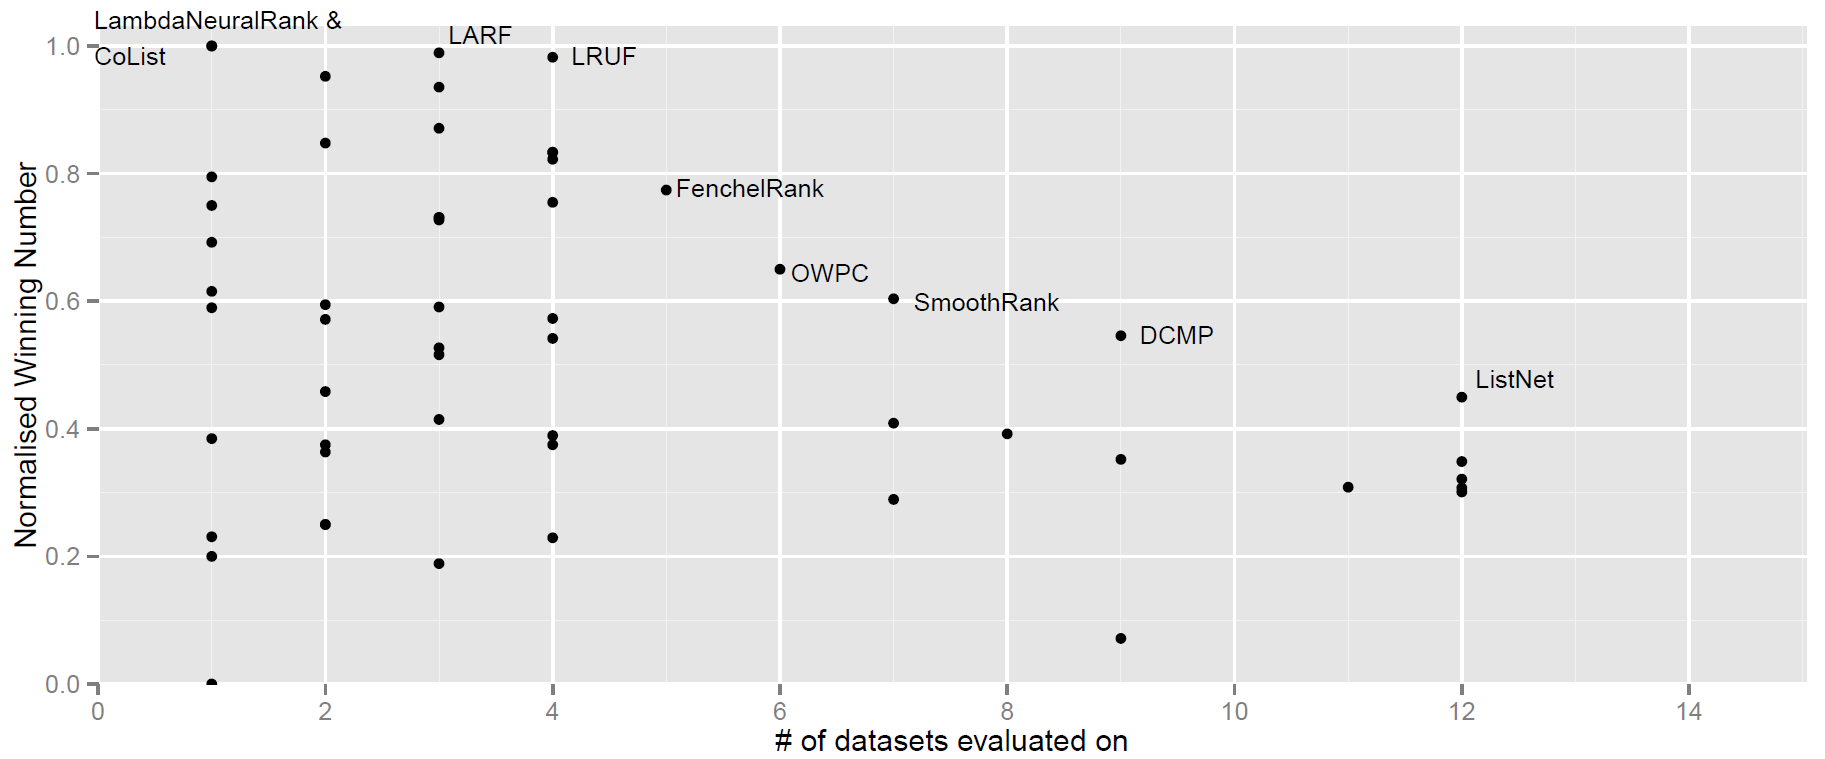
\includegraphics[scale=0.285]{gfx/ndcg3_winnum}
\caption{\acs{NDCG}@3 comparison of Learning to Rank methods}
\label{fig:normalised_winning_number_NDCG3}
\end{figure}

LambdaNeuralRank and CoList both acquired a perfect \ac{NWN} score of 1.0 by beating all other algorithms on one dataset, with LambdaNeuralRank winning on the AOL dataset and CoList winning on Yahoo Set 2. LARF and LRUF both scored very high scores of near 1.0 on three of the LETOR 3.0 data sets, which can be said to have a higher degree of certainty on the methods' performance because they are validated on three data sets which in addition are more relevant data sets than AOL and Yahoo Set 2 because there are more evaluation results available for the LETOR 3.0 data sets (see Table \ref{tab:ltr_methods_used}). FenchelRank, OWPC, SmoothRank, DCMP and ListNet are in that order increasingly lower in \ac{NWN}, but increasingly higher in number of data sets that they are evaluated on, resulting in a higher degree of certainty on the accuracy of the algorithms.\\

LambdaNeuralRank, CoList, LARF, LRUF, OWPC and DCMP evaluation results are all based on one study, therefore are subjected to the risk of one overly optimistic study producing those results. FenchelRank evaluation result are based combined result from two studies, although those studies have overlap in authors. SmoothRank and ListNet have the most reliable evaluation result source, as they were official LETOR baseline runs.  

\subsection{NDCG@5}
Figure \ref{fig:normalised_winning_number_NDCG5} shows the performance of Learning to Rank methods for the \ac{NDCG}@5 metric. Table \ref{tab:raw_data_norm_winnum_NDCG5} in Appendix \ref{app:norm_winnum_NDCG5} provides the raw Normalised Winning Number data for the Learning to Rank methods.\\

\begin{figure}[!h]
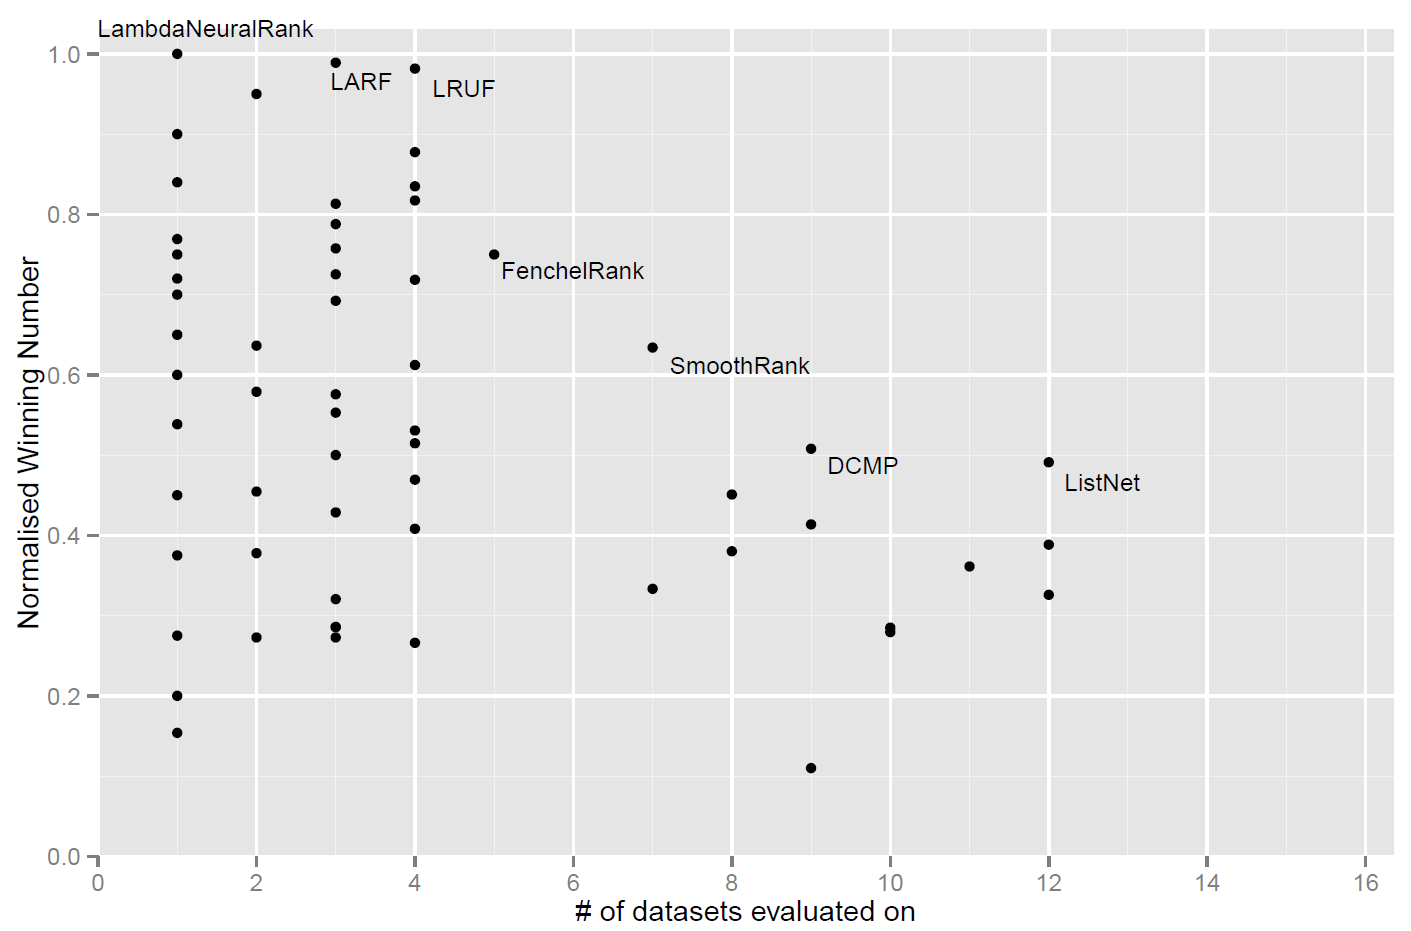
\includegraphics[scale=0.285]{gfx/ndcg5_winnum}
\caption{\acs{NDCG}@5 comparison of Learning to Rank methods}
\label{fig:normalised_winning_number_NDCG5}
\end{figure}

LambdaNeuralRank again beat all other methods solely with results on the AOL dataset scoring a \ac{NWN} of 1.0. LARF, LRUF, FenchelRank, SmoothRank, DCMP and ListNet are from left to right evaluated on an increasing number of data sets, but score decreasingly well in terms of \ac{NWN}. These results are highly in agreement with the \ac{NDCG}@3 comparison. The only modification compared to the \ac{NDCG}@3 comparison being that OWPC did show to be a method for which there were no methods performing better on both axes in the \ac{NDCG}@5 comparison, but not in the \ac{NDCG}@3 comparison. Like in the \ac{NDCG}@3 comparison, SmoothRank and ListNet can be regarded as most reliable results because the evaluation measurements for these methods are based on LETOR official baselines.

\subsection{NDCG@10}
Figure \ref{fig:normalised_winning_number_NDCG10} shows the performance of Learning to Rank methods for the \ac{NDCG}@10 metric. Table \ref{tab:raw_data_norm_winnum_NDCG10} in Appendix \ref{app:norm_winnum_NDCG10} provides the raw Normalised Winning Number data for the Learning to Rank methods.\\

\begin{figure}[!h]
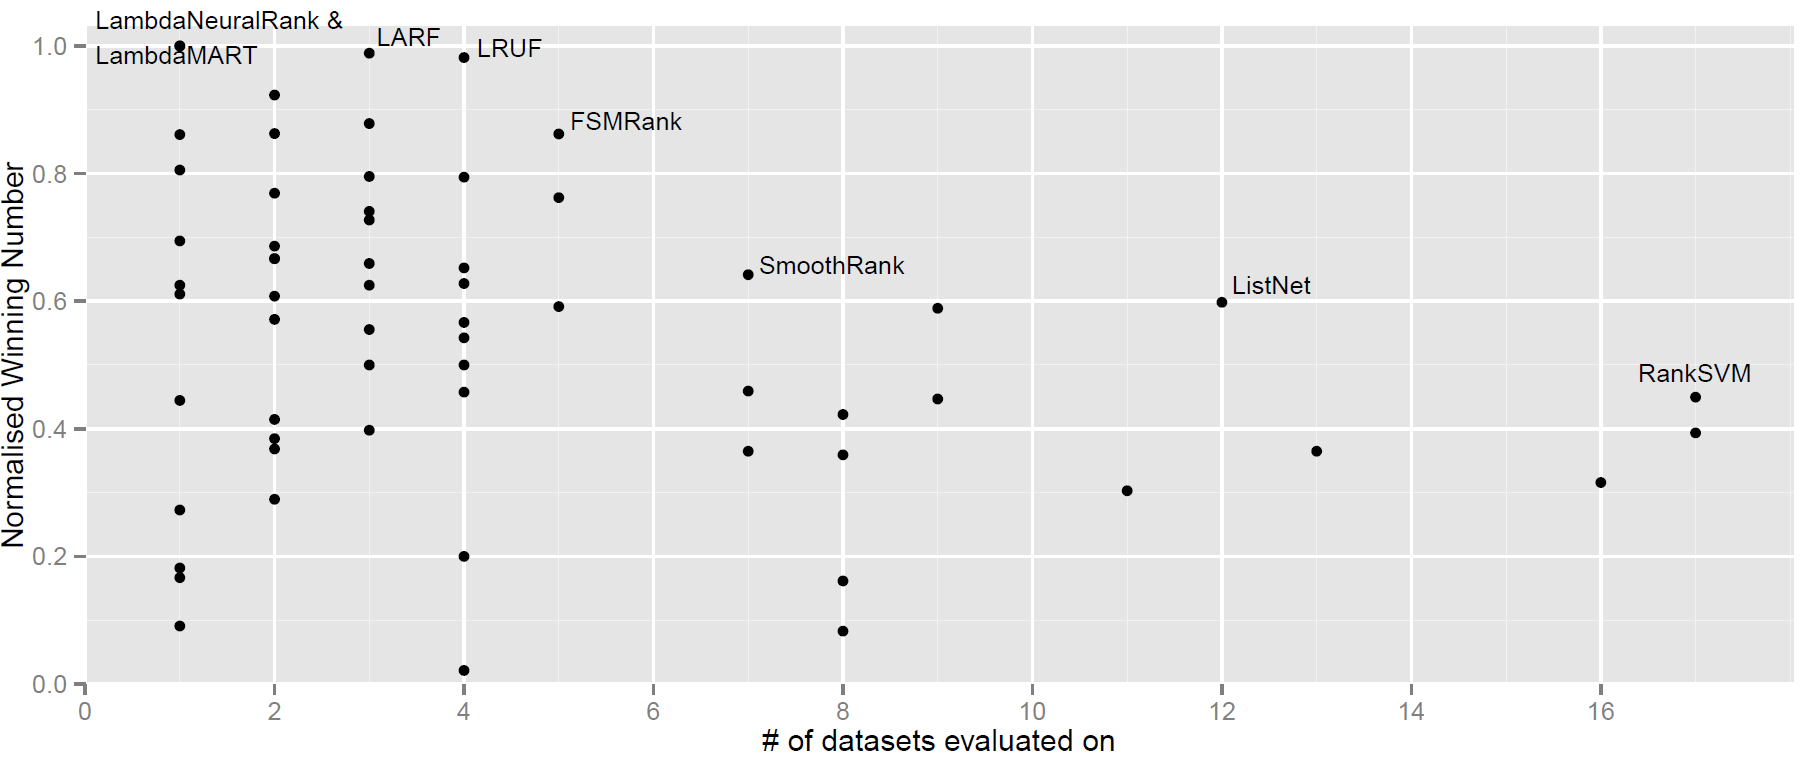
\includegraphics[scale=0.285]{gfx/ndcg10_winnum}
\caption{\acs{NDCG}@10 comparison of Learning to Rank methods}
\label{fig:normalised_winning_number_NDCG10}
\end{figure}

LambdaMART and LambdaNeuralRank score a \ac{NWN} of 1.0 on the \ac{NDCG}@10 comparison. For LambdaNeuralRank these results are again based on AOL dataset measurements. LambdaMART showed the highest \ac{NDCG}@10 performance for the MSLR-WEB10k dataset. The set of algorithms for which there is no other algorithm with both a higher \ac{NWN} and number of data sets evaluated on is partly in agreement with those for the \ac{NDCG}@3 and \ac{NDCG}@5 comparisons: {LARF, LRUF, FSMRank, SmoothRank, ListNet, RankSVM}. SmoothRank and FSMRank were not present in this set for the \ac{NDCG}@3 and \ac{NDCG}@5 comparison, but were close by, as can be seen in Tables \ref{tab:raw_data_norm_winnum_NDCG3} and \ref{tab:raw_data_norm_winnum_NDCG5} in the Appendices. DCMP is not in the set in contrast with the \ac{NDCG}@3 and \ac{NDCG}@5 comparison.

\subsection{MAP}
Figure \ref{fig:normalised_winning_number_map} shows the performance of Learning to Rank methods for the \ac{MAP} metric. Table \ref{tab:raw_data_norm_winnum_map} in Appendix \ref{app:norm_winnum_map} provides the raw \ac{NWN} data for the Learning to Rank methods.\\

\begin{figure}[!h]
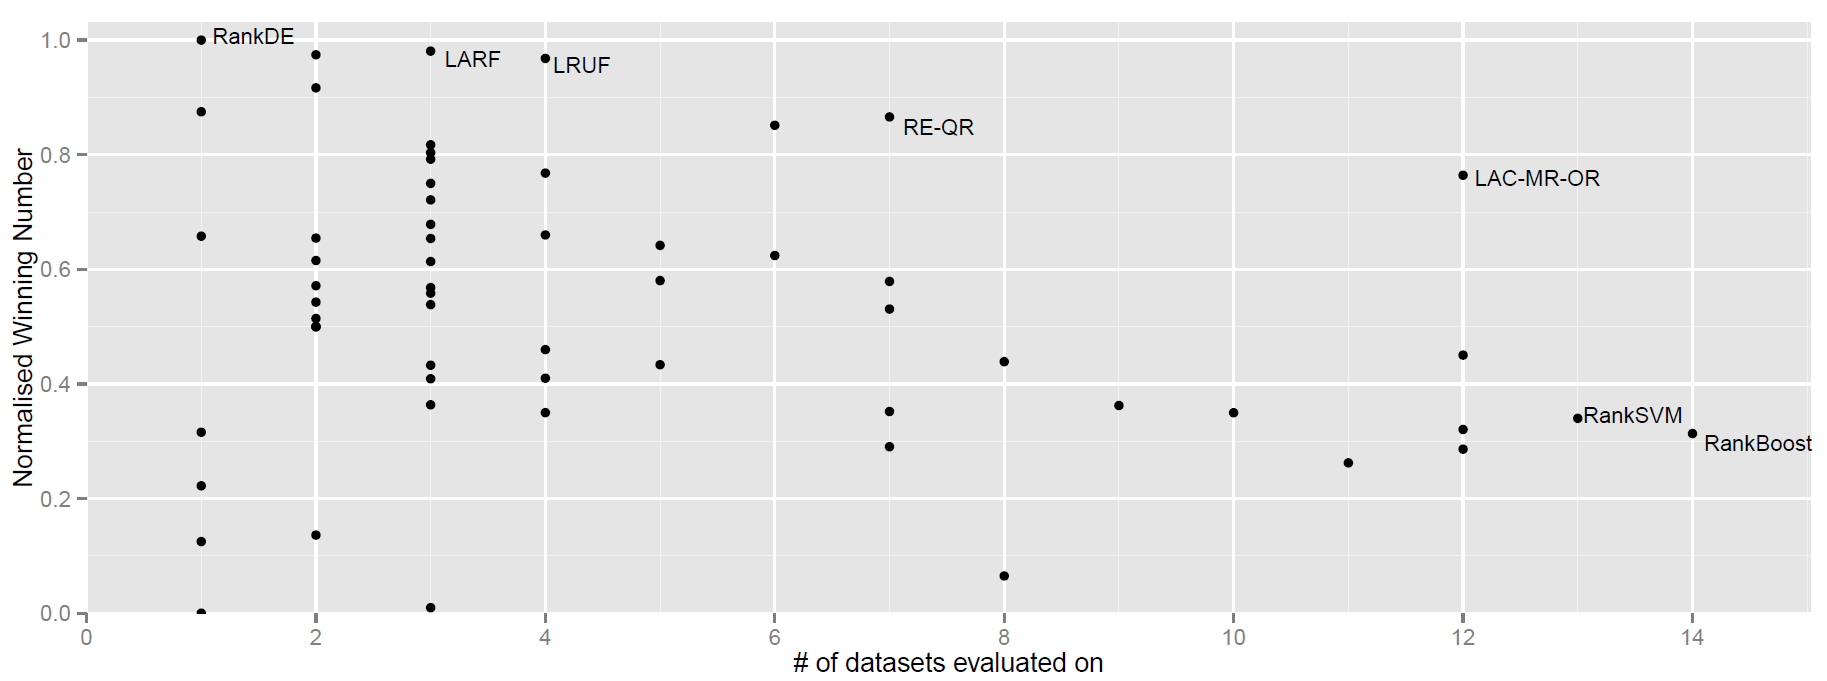
\includegraphics[scale=0.285]{gfx/map_winnum}
\caption{\acs{MAP} comparison of Learning to Rank methods}
\label{fig:normalised_winning_number_map}
\end{figure}

Where comparisons on the \ac{NDCG}-metric at different cut-off points where highly in agreement in terms of the best performing algorithms, the comparison in terms of \ac{MAP} shows different results. RankDE scores a \ac{NWN} of 1.0 on one dataset, like LambdaNeuralRank did on for all \ac{NDCG}-comparisons. In contrast to LambdaNeuralRank, RankDE achieved this highest score on the LETOR 2.0 TD2003, a dataset on which many methods are evaluated.\\

LARF and LRUF score very high \ac{NWN} scores, but based on only relatively few data sets, just as in the \ac{NDCG}-comparisons. Notable is that SmoothRank and ListNet, which showed both high accuracy and high certainty on all \ac{NDCG}-comparisons, are not within the best performing methods in the \ac{MAP}-comparison. A deeper look in the raw data Tables \ref{tab:raw_data_norm_winnum_NDCG3} to \ref{tab:raw_data_norm_winnum_map} in Appendices \ref{app:norm_winnum_NDCG3} to \ref{app:norm_winnum_map} shows that LAC-MR-OR is evaluated on many more data sets for \ac{MAP} compared to \ac{NDCG}, which resulted in LAC-MR-OR obtaining equal certainty to ListNet with a higher \ac{NWN}. SmoothRank performed a \ac{NWN} of around 0.53 over 7 data sets, which is still good in both certainty and accuracy, but not among the top methods. RE-QR is one of the best performers in the \ac{MAP}-comparison with a reasonable amount of benchmark evaluations. No reported \ac{NDCG} performance was found in the literature study for RE-QR. There is a lot of certainty on the accuracy of RankBoost and Rank\ac{SVM} as both models are evaluated on the majority of data sets included in the comparison for the \ac{MAP}-metric, but given their \ac{NWN} it can said that both methods are not within the top performing Learning to Rank methods.

\subsection{Cross-metric}
Figure \ref{fig:normalised_winning_number_all} shows the \ac{NWN} as function of \ac{IWN} for the methods described in Table \ref{tab:ltr_methods_used}. Table \ref{tab:raw_data_norm_winnum_all} in Appendix \ref{app:norm_winnum_all} provide the raw data plotted in Figure \ref{fig:normalised_winning_number_all}.\\

\begin{figure}[!h]
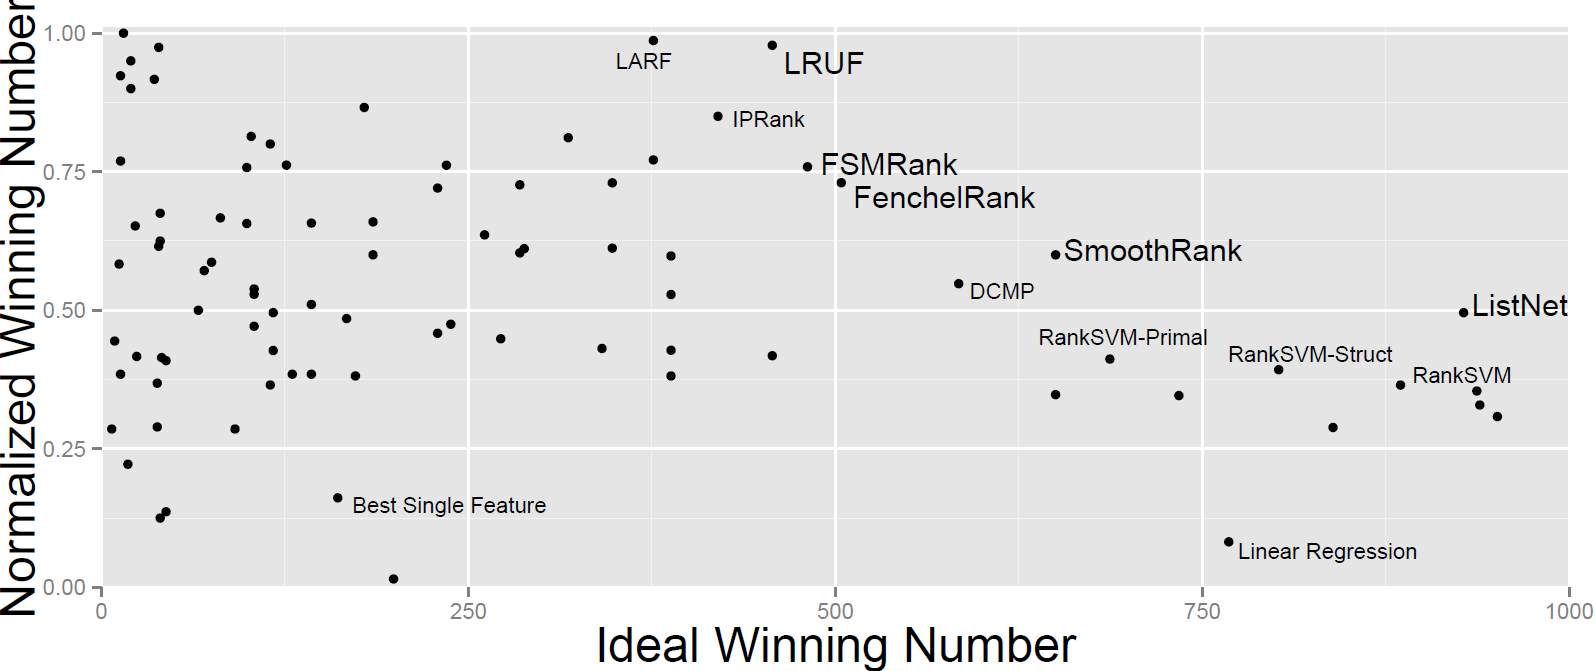
\includegraphics[scale=0.33]{gfx/combined_normalized_winnum}
\caption{Cross-benchmark comparison of Learning to Rank methods}
\label{fig:normalised_winning_number_all}
\end{figure}

The cross-metric comparison is based on the \ac{NDCG}@3, \ac{NDCG}@5, \ac{NDCG}@10 and \ac{MAP} comparisons combined, which justifies analysing the comparison more thoroughly. Figure \ref{fig:normalised_winning_number_all} labels the algorithms with no other algorithm having a higher value on both the horizontal axis and vertical axis, but also labels the algorithms with exactly one algorithm having a higher value on both axes with smaller font size. In addition, Linear Regression and the ranking method of simply sorting on the best single feature are labelled as baselines.\\

LRUF, FSMRank, FenchelRank, SmoothRank and ListNet showed to be the methods that have no other method superior to them in both \ac{IWN} and \ac{NWN}. LRUF is the only method that achieved this in all \ac{NDCG} comparisons, the \ac{MAP} comparison as well as the cross-metric comparison. With FenchelRank, FSMRank, SmoothRank and ListNet being among the top performing methods in all \ac{NDCG} comparisons as well as in the cross-metric comparison, it can be concluded that the cross-metric results are highly defined by the \ac{NDCG} performance as opposed to the \ac{MAP} performance. This was to be expected, because the cross-metric comparison input data of three \ac{NDCG} entries (@3, @5, and @10) enables it to have up to three times as many as many weight as the \ac{MAP} comparison.\\

LARF, \ac{IP}Rank and DCMP and several variants of Rank\ac{SVM} performed very well on the cross-metric comparison, with all having only one method in its top right quadrant. LARF also performed among the top methods on the \ac{NDCG} and \ac{MAP} comparisons and DCMP was a top performer in a few of the \ac{NDCG} comparisons.\\

C-CRF, DirectRank, FP-Rank, RankCSA, LambdaNeuralRank and VFLR all have near-perfect \ac{NWN} measures, but have low \ac{IWN} measures. Further evaluation runs of these methods on benchmark data sets that they are not yet evaluated on are desirable. The DirectRank paper \cite{Tan2013} shows that the method  is evaluated on more data sets than the number of data sets that we included evaluation results for in this meta-analysis. Some of the DirectRank measurements could not be used because measurements on some data sets were only available in graphical form and not in raw data.\\

LAC-MR-OR and RE-QR showed very good ranking accuracy in the \ac{MAP} comparison on multiple data sets. Because LAC-MR-OR is only evaluated on two data sets for \ac{NDCG}@10 and RE-QR is not evaluated for \ac{NDCG} at all, LAC-MR-OR and RE-QR are not within the top performing methods in the cross-metric comparison. 

\section{Limitations}
In the \ac{NWN} calculation the weight of each benchmark on the total score is determined by the number of evaluation measurements on this benchmark. By calculating it in this way, we implicitly make the assumption that the Learning to Rank methods are (approximately) distributed uniformly over the benchmarks, such that the average Learning to Rank method tested are approximately equally hard for each data set. It could be the case however that this assumption is false and that significantly more accurate Learning to Rank methods are evaluated on some data sets than on other data sets. \\

A second limitation is that the data sets on which Learning to Rank methods have been evaluated can not always be regarded a random choice. It might be the case that some researchers chose to publish results for exactly those benchmark data sets that showed the most positive results for their Learning to Rank method.\\

Another limitation is that our comparison methodology relies on the correctness of the evaluation results found in the literature search step. This brings up a risk of overly optimistic evaluation results affecting our NWN results. Limiting the meta-analysis to those studies that report comparable results on one of the baseline methods of a benchmark set reduces this limitation but does not solve it completely. By taking IWN into account in Figure \ref{fig:normalised_winning_number_all} we further mitigate this limitation, as IWN is loosely related with the number of studies that reported evaluation results for an algorithm.\\

Our comparison regarded evaluation results on \ac{NDCG}@{3, 5, 10} and \ac{MAP}. By making the decision to include \ac{NDCG} at three cut-off points and only a single \ac{MAP} entry, we implicitly attain a higher weight for \ac{NDCG} compared to \ac{MAP} on an analysis that combines all measurements on the four metrics. This implicit weighting could be regarded as arbitrary, but the number of algorithm evaluation results gained by this makes it a pragmatic approach. Note that another implicit weighting lies in the paper dimension. Hence, the higher number of evaluation results specified in a paper, the higher the influence of this paper on the outcome of the analysis. This implicit weighting is not harmful to the validity of our comparison, as papers with a large number of evaluation results are more valuable than papers with a few evaluation results. In addition, papers with a high number of evaluation results are not expected to be less reliable than papers with fewer evaluation results.

\section{Conclusions}
We proposed a new way of comparing learning to rank methods based on sparse evaluation results data on a set of benchmark datasets. Our comparison methodology comprises of two components: 1) \ac{NWN}, which provides insight in the ranking accuracy of the learning to rank method, and 2) \ac{IWN}, which gives insight in the degree of certainty concerning the performance of the ranking accuracy.\\

Based on this this new comparison approach for a set of sparse evaluation results, we will now look back on the first research question of the thesis.
\begin{description}
\item[RQ1] What are the best performing Learning to Rank algorithms in terms of ranking accuracy on relevant benchmark data sets?\\
\end{description}
Although no closing arguments can be formulated on which Learning to Rank methods are most accurate, a lot of insight has been gained with the cross-benchmark comparison on which methods tend to perform better than others.\\

Based on our literature search for evaluation results on well-known benchmarks collections, a lot of insight has been gained with the cross-benchmark comparison on which methods tend to perform better than others. However, no closing arguments can be formulated on which learning to rank methods are most accurate. LRUF, FSMRank, FenchelRank, SmoothRank and ListNet were the learning to rank algorithms for which it holds that no other algorithm produced more accurate rankings with a higher degree of certainty of ranking accuracy. From left to right, the ranking accuracy of these methods decreases while the certainty of the ranking accuracy increases.\\

LRUF, FSMRank, FenchelRank, SmoothRank and ListNet were the Learning to Rank algorithms for which it holds that no other algorithm produced more accurate rankings with a higher degree of certainty of ranking accuracy. From left to right, the ranking accuracy of these methods decreases while the certainty of the ranking accuracy increases. For more definite conclusions on the relative performance of these five methods, more evaluation runs on are desirable for the methods on the left side on the list on benchmark data sets that these methods have not yet been evaluated on.\\

More evaluation runs are needed for the methods on the left side of Figure \ref{fig:normalised_winning_number_all}. Our work contributes to this by identifying promising learning to rank methods that researchers could focus on in performing additional evaluation runs.\\

In the following chapters of this thesis, concerning parallel execution of the Learning to Rank training phase, the scope will be limited to the five methods that turned out to be superior Learning to Rank methods in terms of ranking accuracy and certainty about this ranking accuracy: LRUF, FSMRank, FenchelRank, SmoothRank and ListNet. Although it can not be concluded that these methods are inarguably the most accurate Learning to Rank methods, a strong presumption has been raised that these five Learning to Rank are accurate ranking methods.\\